\section{Affine Copies and the Self Similarity Property}

    %Patterns in Data sets
    %Def Affine Copy
    %Def Measure-Universal
    %State Erdos Conjecture
    %History/Context for Erdos Conjecture, 
        %Proposed Year
        %Who are main researchers?
        %What is current Progress?
    %Def Topological-Universal
    %Propose Analogous Theorem
    %Outline Paper Sections ahead
        %Measure ideas:
        %Topology ideas:
        %Gap Lemma
        %Main Thm
        %Multi-Dim Thm

One of the more popularly known results from math is the the Mandelbrot set fractal.  In some senses fractals can be very general objects that are considered to have fractional dimensions.  This definition can be very general but by that same token, may not always capture some of the inherent geometry of some fractal type objects. Some objects with fractional dimensions have a self-similar property, and some self-similar objects have fractional dimension.  For the scope of this paper, we will not be discussing dimension. However we will investigate the notion of self-similarity. 

We can now start by defining \textit{affine transformations} or \textit{affine copies}.
\begin{definition}[Affine copy]
    An \underline{affine copy} of a set $A$ is a scaled and translated set $A'$ such that for some $\lambda\neq 0, \lambda \in \R$ and $t \in \R$,  $$A' = \{\lambda a + t : a \in A\}.$$
\end{definition}

Even one dimensional objects can have this self-similar property. Take for example the middle Third Cantor set.  The middle third Cantor set is defined by recursively removing the open middle third interval of the previous remaining closed intervals.  Explicitly this can be constructed using countable intersection.  

\begin{example}[The Middle Third Cantor Set]\label{middleThirdCantor}
    $$\mathcal{C} = [0,1] \setminus \bigcup_{n=0}^\infty\bigcup_{k=0}^{3^n-1}\left(\frac{3k+1}{3^{n+1}},\frac{3k+2}{3^{n+1}}\right)$$
\end{example}

This set in particular exhibits this self-similar property because each level is a scaled copy of the entire object.  The following figure shows the first seven intervals removed.  

\begin{figure}[h]
    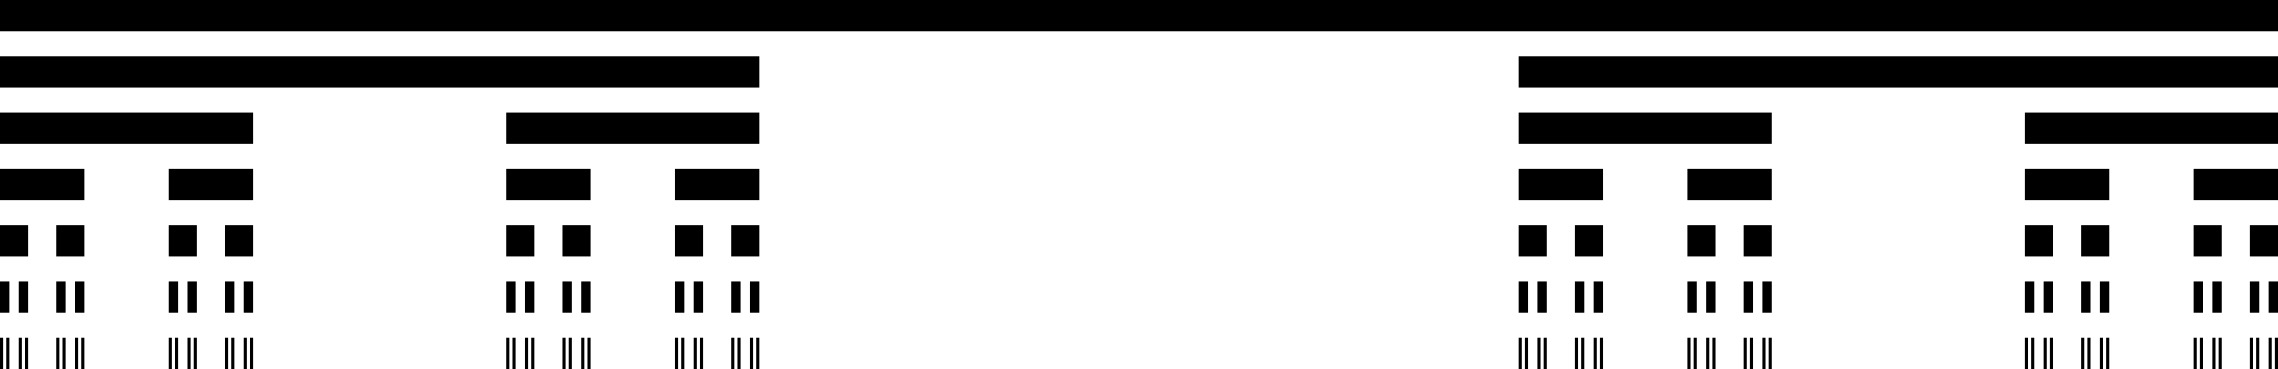
\includegraphics[width=0.8\textwidth]{Content/Images/Cantor_set_in_seven_iterations.jpg}
    \centering
    \caption{The first seven iterations of the middle third Cantor Set.}
\end{figure}
In a general sense, we can take a set, then dilate and translate a copy of it. 

\begin{definition}[Dilation]
    Let $r>0$ and $a \in \R$.  The \underline{dilation} on $\R$ with ratio $r$ and center $a$ is the function $f: \R \to \R$ given by $$f(x)= rx + (1-r) a.$$
\end{definition}

Now we consider the 

\begin{definition}[Self-Similar Set]
    A set $A$ is self-similar if it is the invariant set of an iterated function system. 
\end{definition}

Admittedly this is an abstract definition, so we come back to the Cantor set from earlier.  
\begin{claim}The Cantor set is self-similar.   
\end{claim}
\begin{proof}
    Recall the definition of the Cantor set, as the iterated removal of the middle third.      
    $$\mathcal{C} = [0,1] \setminus \bigcup_{n=0}^\infty\bigcup_{k=0}^{3^n-1}\left(\frac{3k+1}{3^{n+1}},\frac{3k+2}{3^{n+1}}\right)$$

    Here we notice that for the first removal, $n = 0$, we are left with the left and right portion of the Cantor set.  Specifically the left side is a translated copy of the right side:

    $$\left\{ \left[0,\frac{1}{3}\right] \setminus \bigcup_{n=0}^\infty\bigcup_{k=0}^{3^n-1}\left(\frac{3k+1}{3^{n+1}},\frac{3k+2}{3^{n+1}}\right) \right\} + \frac{2}{3} = \left[\frac{2}{3},1\right] \setminus \bigcup_{n=0}^\infty\bigcup_{k=0}^{3^n-1}\left(\frac{3k+1}{3^{n+1}},\frac{3k+2}{3^{n+1}}\right).$$

    We note that this happens at every level where 

\end{proof}
\begin{definition}[Iterated Function System]
    An iterated function system is a finite set of contraction mappings on a complete metric space.  Symbolically, we write this as, for some $N \in \N$,
    $$\{f_i:X \to X \vert i = 1,2,\dots, N\}, $$
\end{definition}

The invariant set under this iterated function system is a self similar set.